\section{Results and Analysis}
\label{sec:results}

Validation numbers decided every step; the test numbers below come from the single final
evaluation. Where both are given, they agree within 0.2 points of top-1 and 0.003 of AUC.

\subsection{The scale leak (H1)}
\label{sec:res-leak}

\IfFileExists{figures/fig_prefix_example.pdf}{%
\begin{figure}[t]
\centering
\includegraphics[width=\linewidth]{fig_prefix_example}
\caption{One validation drawing and the three inputs for its first 25\% of ink. Dots are the
model's input points. In the full frame the prefix is visibly small; after rescaling by its own
box, the gaps between stored points reveal the magnification; uniform resampling evens them out.}
\label{fig:prefix}
\end{figure}}{}

% Generated by paper/make_assets.py from reports/final_v1_test, reports/leak_v1, reports/followup_v1. Do not edit by hand.
\begin{table}[t]
\centering
\caption{Claim 1, the scale leak. Top-1 accuracy (\%) at each ink fraction on the test split
(every test drawing, mean of seeds 42 and 43). Early: mean over 10, 25 and 50\% ink. $\Delta$: early
top-1 minus the same model with \emph{prefix} input, in points. The last column is the same early
top-1 on validation (1{,}000 drawings per class), where every decision was taken.}
\label{tab:leak}
\setlength{\tabcolsep}{3.5pt}
\begin{tabular}{llrrrrrrrr}
\toprule
& & \multicolumn{5}{c}{Top-1 at ink fraction (test)} & \multicolumn{2}{c}{Early (test)} & Early \\
\cmidrule(lr){3-7}\cmidrule(lr){8-9}
Model & Input & 10\% & 25\% & 50\% & 75\% & 100\% & top-1 & $\Delta$ & (val) \\
\midrule
GRU & prefix & 10.1 & 28.0 & 55.0 & 73.9 & 79.0 & 31.0 & -- & 31.2 \\
GRU & full\_bbox (leaky) & 23.6 & 41.5 & 62.2 & 76.0 & 80.0 & 42.4 & $+11.4$ & 42.5 \\
GRU & uniform & 8.6 & 26.5 & 54.4 & 73.4 & 78.3 & 29.8 & $-1.2$ & 29.9 \\
\midrule
CNN & prefix & 8.3 & 28.6 & 58.9 & 78.4 & 83.9 & 31.9 & -- & 32.0 \\
CNN & full\_bbox (leaky) & 23.4 & 44.1 & 66.7 & 80.5 & 84.8 & 44.7 & $+12.8$ & 44.8 \\
\bottomrule
\end{tabular}
\end{table}


\begin{figure}[t]
\centering
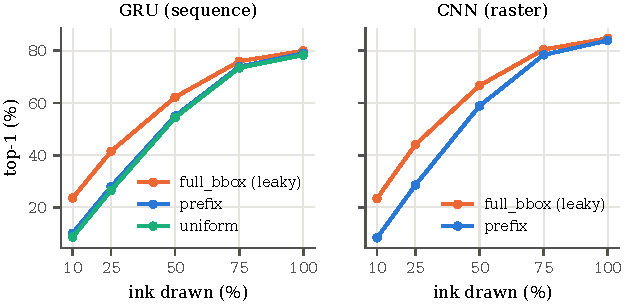
\includegraphics[width=\linewidth]{fig_leak}
\caption{Test top-1 against ink drawn (every test drawing, mean of two seeds). The leaky
full-frame input gains most when little is drawn; at 100\% ink all inputs see the same drawing.}
\label{fig:leak}
\end{figure}

Table~\ref{tab:leak} and Fig.~\ref{fig:leak} confirm the first part of H1. Keeping the finished
drawing's frame raises early top-1 by 11.4 points for the GRU and 12.8 points for the CNN on test,
and at 10\% ink it raises top-1 from 10.1\% to 23.6\% (GRU) and from 8.3\% to 23.4\% (CNN). The gain shrinks as
ink grows, as it should: at 100\% ink the two inputs are identical, and the remaining
0.9--1.0-point difference comes from training on different inputs. A model evaluated with the
finished drawing's frame would thus overstate early recognition several times over.

The second part, a residual leak in per-prefix inputs, took two attempts. Our pre-registered fix
resampled each stroke at even spacing but kept its end points; it cost 1.4 points of early top-1
on validation, more than the one-point margin we had set, so the rule kept \emph{prefix} input.
A separate audit then attacked the inputs directly. Reading the coordinate lattice of a rescaled
prefix recovers its size relative to the finished drawing within 3\% for 90.2\% of validation
prefixes, against 33.7\% for always guessing ``full size'' and 87.4\% on prefixes below 0.9 of the
full size. Using only stroke end points, which the first fix kept, still recovers it for 48.6\%.
After uniform resampling (Sect.~\ref{sec:method-norm}) the attack succeeds for 0.01\%. Regressors
trained to predict the log size ratio (gradient boosting on sequence features, a small CNN on
$64\times64$ rasters) reach $R^2 = 0.754$ on stored prefixes, 0.529 after uniform resampling and
0.501 on rasters. Part of this is legitimate, since shape alone says something about size: on two
classes for which we cut prefixes from the raw strokes and only then simplified them, the clean
inputs reach $R^2 \approx 0.55$. Against these clean references, stored sequences exceed by 0.24,
resampled sequences by 0.10 and rasters by 0.08. We therefore
report the GRU's early numbers with uniform input. It loses 1.2 points of early top-1 to
\emph{prefix} input on test (29.8 against 31.0) and 0.005 of stopping AUC on validation. This is an
upper bound on what the residual leak was worth to the GRU, because resampling also cuts corners
(raster IoU before and after: median 0.87). It is roughly ten times smaller than the full-frame
effect. For the CNN the residual is not measured in accuracy (Sect.~\ref{sec:limits}).

\subsection{When to guess (H2)}
\label{sec:res-anytime}

% Generated by paper/make_assets.py from reports/followup_v2_anytime, reports/anytime_v1_two_seeds. Do not edit by hand.
\begin{table}[t]
\centering
\caption{Claim 2a on validation (evaluation half, 100 drawings per class): area under the
accuracy--earliness frontier (AUC, higher is better) of the stopping policy named first (A) and
second (B). Upper block: GRU with uniform resampling, the leak-free sequence setting. $^\dagger$One
seed. Seed-to-seed range of a condition is at most 0.0026.}
\label{tab:ablation}
\setlength{\tabcolsep}{4pt}
\begin{tabular}{p{5.6cm}rrrc}
\toprule
Comparison (A vs B) & AUC A & AUC B & A $-$ B & Seeds \\
\midrule
Full method (head + consistency + 2 prefixes) vs baseline & 0.4467 & 0.4594 & $-0.0126$ & 2 \\
Confidence head vs max softmax, same classifier & 0.4467 & 0.4471 & $-0.0004$ & 2 \\
With vs without consistency loss & 0.4467 & 0.4521 & $-0.0054$ & 2 \\
Two prefixes per drawing alone vs baseline & 0.4523 & 0.4594 & $-0.0071$ & 2 \\
Margin vs max softmax (baseline model) & 0.4598 & 0.4594 & $+0.0004$ & 2 \\
$2\times$ steps, same compute: method vs baseline$^\dagger$ & 0.4746 & 0.4838 & $-0.0092$ & 1 \\
Baseline $2\times$ vs $1\times$ steps$^\dagger$ & 0.4838 & 0.4594 & $+0.0244$ & 1 \\
\midrule
GRU, prefix input: method vs baseline & 0.4548 & 0.4648 & $-0.0099$ & 2 \\
\midrule
CNN: method vs baseline & 0.4938 & 0.4999 & $-0.0061$ & 2 \\
\bottomrule
\end{tabular}
\end{table}

% Generated by paper/make_assets.py from reports/final_v1_test/results.json. Do not edit by hand.
\begin{table}[t]
\centering
\caption{Claims 2a and 2b on the test split (500 drawings per class, 50{,}000 drawings), thresholds
from the validation calibration half. AUC and end accuracy (\%, answer at the end of the drawing):
mean of two seeds. Risk control with target gap $\epsilon$: worst realised gap over the two seeds
(\%), then mean accuracy (\%) and mean ink used when answering. $^\ast$Realised gap above
$\epsilon$ for one seed. Over every run, stopping score and target, 38 of 40 are met.}
\label{tab:test_anytime}
\setlength{\tabcolsep}{2.6pt}
\begin{tabular}{lllrrrrrrrr}
\toprule
& & & & End & \multicolumn{3}{c}{$\epsilon = 2\%$} & \multicolumn{3}{c}{$\epsilon = 5\%$} \\
\cmidrule(lr){6-8}\cmidrule(lr){9-11}
Model & Training & Stopping score & AUC & acc. & gap & acc. & ink & gap & acc. & ink \\
\midrule
GRU & baseline & max softmax & 0.458 & 78.5 & 1.93 & 77.2 & 0.839 & 4.85 & 75.1 & 0.766 \\
GRU & baseline & margin & 0.458 & 78.5 & 1.90 & 77.2 & 0.840 & 5.04$^\ast$ & 74.9 & 0.765 \\
GRU & method & head & 0.446 & 75.6 & 1.86 & 74.6 & 0.838 & 4.46 & 72.7 & 0.770 \\
GRU & method & max softmax & 0.447 & 75.6 & 1.91 & 74.6 & 0.842 & 4.44 & 72.7 & 0.771 \\
\midrule
CNN & baseline & max softmax & 0.498 & 84.0 & 1.79 & 83.1 & 0.808 & 4.72 & 81.0 & 0.742 \\
CNN & baseline & margin & 0.497 & 84.0 & 1.84 & 83.1 & 0.806 & 4.45 & 81.1 & 0.744 \\
CNN & method & head & 0.491 & 82.5 & 1.94 & 81.6 & 0.810 & 4.76 & 79.6 & 0.743 \\
CNN & method & max softmax & 0.491 & 82.5 & 1.80 & 81.6 & 0.809 & 4.75 & 79.5 & 0.741 \\
\bottomrule
\end{tabular}
\end{table}


H2 is rejected. At equal compute, the method's stopping AUC is lower than that of the max-softmax
baseline in every comparison: by 0.013 for the uniform GRU on validation and 0.012 on test
(0.446 against 0.458), by 0.006 and 0.007 for the CNN (test 0.491 against 0.498), and by 0.010 for
the GRU with prefix input (Tables~\ref{tab:ablation} and~\ref{tab:test_anytime}). Seed-to-seed
ranges are below 0.003, so the sign is not in doubt. The learned confidence adds nothing over the
max softmax of the same classifier ($-0.0004$ on validation, $-0.0003$ on test): the head
recovers, at best, what the softmax already knows. The margin is equally close to the max
softmax ($+0.0004$), and a rule that answers after a fixed number of strokes is far behind (AUC
0.288 against 0.459 for the uniform GRU).

The ablations place the loss in the classifier, not the stopping score. Training on two prefixes
per drawing, with the head but without consistency, costs 0.007; adding the consistency loss
costs another 0.005. At a fixed number of steps, two prefixes per drawing means each drawing is
visited four times instead of eight, and the baseline is clearly under-trained: doubling its steps
adds 0.024 AUC and raises its end accuracy from 78.6\% to 81.6\%. An exploratory run that trained
the method twice as long (prefix input) had beaten the 1$\times$ baseline by 0.011, but its own max
softmax did the same (+0.011): the gain came from longer training. With both sides doubled, the
method still loses by 0.009 ($-0.008$ for its own max softmax).

\begin{figure}[t]
\centering
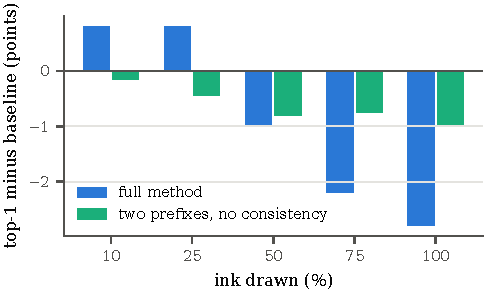
\includegraphics[width=0.75\linewidth]{fig_early_late}
\caption{Validation top-1 of the method and of two-prefix training without consistency, minus the
uniform-GRU baseline, at each ink fraction (two seeds). Consistency buys early accuracy with late
accuracy.}
\label{fig:earlylate}
\end{figure}

Fig.~\ref{fig:earlylate} shows what the consistency loss does. It improves top-1 by 0.8 points at
10\% and 25\% ink (9.6\% against 8.8\% at 10\%) and lowers it by 1.0 to 2.8 points from 50\% ink
on (75.7\% against 78.5\% at the end). Two prefixes without consistency are slightly worse at
every fraction. Pulling the short prefix toward the long one does make early predictions better,
as intended, but most accuracy, and hence most of the AUC, is earned after half the ink. We do not
know why late accuracy drops; two explanations we have \emph{not} tested are that the shared
encoder trades capacity toward short prefixes, and that a teacher which is itself often wrong at
mid-drawing propagates its errors.

\begin{figure}[t]
\centering
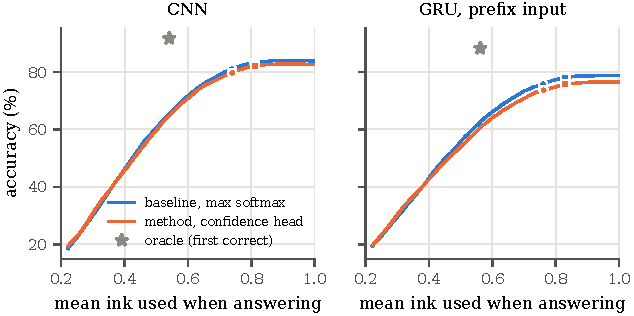
\includegraphics[width=\linewidth]{fig_frontier}
\caption{Accuracy against mean ink used, as the stopping threshold varies (validation evaluation
half, seed 42, prefix input; these are the runs whose full curves were saved). Squares and
circles: thresholds calibrated for $\epsilon = 2\%$ and $5\%$. Star: an oracle answering at the
first correct checkpoint.}
\label{fig:frontier}
\end{figure}

Fig.~\ref{fig:frontier} shows the size of the problem that remains. An oracle that answers at the
first correct checkpoint would be right 88--92\% of the time after 54--57\% of the ink, while the
calibrated threshold rules need 74--84\% of the ink to come within 2--5 points of their final
accuracy.
Neither score identifies the moment an answer becomes right.

\subsection{Stopping with a guaranteed accuracy gap}
\label{sec:res-risk}
Thresholds calibrated on 10{,}000 validation drawings kept the realised accuracy gap below its
target in 38 of 40 test cases (8 runs, 2--3 scores, 2 targets; Table~\ref{tab:test_anytime}). Both
misses use the margin score and exceed the target by little: 2.02\% for $\epsilon = 2\%$ and 5.04\%
for $\epsilon = 5\%$. With 50{,}000 test drawings, the standard error of a 5\% rate is about 0.1
point, so these are within sampling noise of a population gap at the target, which is what the
guarantee bounds. At $\epsilon = 5\%$, max-softmax stopping answers after 74\% of the ink for the
CNN (accuracy 81.0\% against 84.0\% at the end) and 77\% for the GRU (75.1\% against 78.5\%); at
$\epsilon = 2\%$ it needs 81--84\%. The guarantee holds, but the savings are modest: about a
quarter of the ink at a 5\% gap.

\subsection{Coarse-to-fine answers (H3)}
\label{sec:res-hier}

% Generated by paper/make_assets.py from reports/final_v1_test/results.json. Do not edit by hand.
\begin{table}[t]
\centering
\caption{Claim 3, hierarchical answers. Reward area (higher is better) of the answering rule with
each tree, at a precision target chosen on the validation calibration half; mean of two seeds.
Random: the semantic tree's shape with shuffled classes (5 shuffles). Shape: one level of
early-shape clusters. Gain: semantic minus flat. Prec.: realised precision of the semantic rule.}
\label{tab:hierarchy}
\setlength{\tabcolsep}{4pt}
\begin{tabular}{llrrrrrr}
\toprule
Target & Model & semantic & flat & random & shape & Gain & Prec. \\
\midrule
\multicolumn{8}{l}{\emph{Test split}} \\
0.95 & GRU uniform & 0.175 & 0.137 & 0.135 & 0.165 & $+0.038$ & 0.952 \\
0.95 & CNN prefix & 0.234 & 0.190 & 0.193 & 0.228 & $+0.043$ & 0.955 \\
0.90 & GRU uniform & 0.230 & 0.193 & 0.193 & 0.230 & $+0.038$ & 0.904 \\
0.90 & CNN prefix & 0.291 & 0.253 & 0.255 & 0.293 & $+0.038$ & 0.906 \\
\midrule
\multicolumn{8}{l}{\emph{Unseen countries}} \\
0.95 & GRU uniform & 0.172 & 0.132 & 0.131 & 0.159 & $+0.040$ & 0.942 \\
0.95 & CNN prefix & 0.233 & 0.189 & 0.192 & 0.225 & $+0.044$ & 0.943 \\
0.90 & GRU uniform & 0.226 & 0.188 & 0.188 & 0.222 & $+0.038$ & 0.887 \\
0.90 & CNN prefix & 0.289 & 0.250 & 0.252 & 0.288 & $+0.039$ & 0.889 \\
\bottomrule
\end{tabular}
\end{table}


H3 is confirmed (Table~\ref{tab:hierarchy}). At precision 0.95, the semantic tree raises the
reward area from 0.137 to 0.175 for the GRU and from 0.190 to 0.234 for the CNN on test, with
realised precision 0.952--0.956. It answers at 35\% of checkpoints against 23\% for flat answers
(GRU). A tree of the same shape with shuffled classes does no better than flat answers (0.135), so
the gain comes from which classes are grouped, not from having coarse nodes. The shape tree,
however, comes close: 0.165 at precision 0.95, a tie at 0.90 for the GRU (0.2297 against 0.2302), and
slightly ahead at 0.90 for the CNN (0.293 against 0.291). An
everyday-meaning tree is thus a good tree, but we cannot claim it beats one derived from how
drawings start.

\begin{figure}[t]
\centering
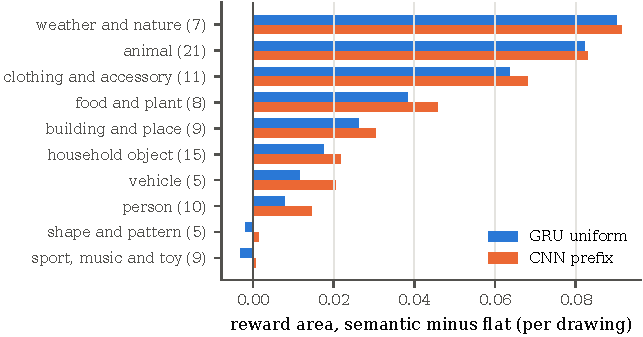
\includegraphics[width=0.75\linewidth]{fig_groups}
\caption{Gain of the semantic tree over flat answers per top-level group (validation evaluation
half, precision 0.95, mean of two seeds; number of classes in brackets).}
\label{fig:groups}
\end{figure}

Fig.~\ref{fig:groups} locates the gain. Weather and nature (+0.09 per drawing), animal (+0.08) and
clothing (+0.06) dominate; the 21 animal classes alone bring 40--44\% of the total gain. Shape and
pattern, and sport, music and toy gain nothing. The classes that gain most are tornado, hurricane,
sweater, jacket, horse, zebra and t-shirt, pairs whose early strokes look alike (spirals, garment
outlines, four-legged bodies) and also share a meaning. Where meaning and early shape coincide, a
group can be named long before the class; where they do not (a cello and a megaphone, a square and
camouflage), the group is no easier than the class. This also explains why the shape tree ties.

\subsection{Recognised and unrecognised drawings}
\label{sec:res-recognized}

% Generated by paper/make_assets.py from reports/analysis_v1/results.json. Do not edit by hand.
\begin{table}[t]
\centering
\caption{Validation AUC differences (A $-$ B) split by the game's \texttt{recognized} flag
(91.9\% of validation drawings are recognized).
Thresholds always come from the whole calibration half; only the evaluation half is split. End
accuracy of the runs analysed: 79.8--88.0\% on recognized
drawings, 27.3--36.3\% on unrecognized ones.
$^\dagger$One seed.}
\label{tab:recognized}
\setlength{\tabcolsep}{4pt}
\begin{tabular}{p{5.2cm}rrr}
\toprule
Comparison (A vs B) & All & Recog. & Unrecog. \\
\midrule
Method vs baseline, GRU uniform & $-0.0126$ & $-0.0121$ & $-0.0139$ \\
Same as above, $2\times$ steps$^\dagger$ & $-0.0092$ & $-0.0088$ & $-0.0097$ \\
Method vs baseline, GRU prefix & $-0.0099$ & $-0.0097$ & $-0.0123$ \\
Method vs baseline, CNN & $-0.0061$ & $-0.0056$ & $-0.0106$ \\
Uniform vs prefix input, GRU (max softmax) & $-0.0054$ & $-0.0071$ & $+0.0054$ \\
\bottomrule
\end{tabular}
\end{table}


Since a recognised drawing stops when the game recognised it, we repeat every comparison on the
two groups (Table~\ref{tab:recognized}). Every method-versus-baseline difference keeps its sign
in both. Unrecognised drawings are a different regime: end accuracy falls to 30--36\% and AUC to
about 0.2. There the uniform input is slightly \emph{better} than prefix input ($+0.005$
against $-0.007$ on recognised drawings); one reading, not tested further, is that the residual
leak helps mainly on recognised drawings.

\subsection{Unseen countries}
\label{sec:res-unseen}

% Generated by paper/make_assets.py from reports/final_v1_test/results.json. Do not edit by hand.
\begin{table}[t]
\centering
\caption{Held-out countries (IN, IT, KR, SA, TH; never seen in training or validation) against the
in-distribution test split. Top-1 (\%) at 10, 50 and 100\% ink on every drawing; AUC and worst
realised gap (\%) at $\epsilon = 5\%$ of max-softmax stopping on 500 drawings per class; mean of two seeds.}
\label{tab:unseen}
\setlength{\tabcolsep}{4pt}
\begin{tabular}{llrrrrr}
\toprule
Model & Set & 10\% & 50\% & 100\% & AUC & gap at 5\% \\
\midrule
GRU uniform & test & 8.6 & 54.4 & 78.3 & 0.458 & 4.85 \\
GRU uniform & unseen & 8.6 & 52.5 & 74.7 & 0.440 & 4.89 \\
\addlinespace
CNN prefix & test & 8.3 & 58.9 & 83.9 & 0.498 & 4.72 \\
CNN prefix & unseen & 8.3 & 57.2 & 80.8 & 0.484 & 4.71 \\
\bottomrule
\end{tabular}
\end{table}


On the five held-out countries (Table~\ref{tab:unseen}), end accuracy drops from 78.3\% to 74.7\%
(GRU) and from 83.9\% to 80.8\% (CNN), but early accuracy is unchanged (8.2--8.6\% at 10\% ink):
what differs between countries is the finished drawing, not its first strokes. Stopping AUC falls
by 0.014--0.019. Thresholds calibrated on validation still met the accuracy-gap target in 15 of 16
cases (one margin miss at 5.06\%), although the guarantee does not formally cover this shift. The
semantic tree's gain over flat answers is the same as in distribution (+0.040 GRU, +0.044 CNN),
but its realised precision falls to 0.941--0.944 for a 0.95 target.

\subsection{An off-the-shelf base model}
\label{sec:res-base}

% Generated by paper/make_assets.py from reports/pretrained_v1*, reports/hierarchy_pretrained_v1, reports/leak_v1. Do not edit by hand.
\begin{table}[t]
\centering
\caption{Off-the-shelf base model, \textbf{validation only} (added after the test split was opened).
Top-1 (\%) at 10 and 100\% ink and early top-1 (10--50\%) on 1{,}000 drawings per class; end accuracy (\%),
AUC and ink used at $\epsilon = 5\%$ of max-softmax stopping, and (Tree) semantic-minus-flat reward area at
precision 0.95, on the evaluation half. Project CNN: the \emph{cnn\_prefix} runs; ResNet-18:
torchvision's network. Mean of two seeds; same training protocol for every row.
$^\ast$Gap target missed for a seed.}
\label{tab:pretrained}
\setlength{\tabcolsep}{3pt}
\begin{tabular}{lrrrrrrrr}
\toprule
Model & Params & 10\% & 100\% & Early & End & AUC & Ink & Tree \\
\midrule
Project CNN & 2.8M & 8.4 & 83.9 & 32.0 & 83.8 & 0.500 & 0.740 & $+0.044$ \\
ResNet-18, scratch & 11.2M & 8.5 & 83.8 & 32.1 & 84.0 & 0.503 & 0.735 & $+0.041$ \\
ResNet-18, ImageNet & 11.2M & 9.0 & 85.0 & 33.1 & 84.9 & 0.512 & 0.723 & $+0.045$ \\
\bottomrule
\end{tabular}
\end{table}


To check that the conclusions do not rest on a small network of our own, we repeated the stopping
and hierarchy evaluations with torchvision's ResNet-18 (Table~\ref{tab:pretrained}, validation only).
Trained from scratch, it matches our CNN (top-1 83.8\% against 83.9\% at the end of the drawing, AUC
0.503 against 0.500) with four times the parameters, so our CNN is not a weak baseline for this
input. ImageNet weights help modestly: +1.1 points of top-1 at the end (85.0\%), +1.2 points of early
top-1 (33.1\% against 32.0\%), and +0.012 AUC, of which +0.009 over the same network from scratch.
Pretraining on photographs thus transfers a little to doodles, but does not change the picture.
The findings on stopping and on the tree hold for the pretrained model (the leak and the learned
stopping method were not re-run with it): the margin is not better than the max softmax
($-0.0015$); the risk-control targets are met for both seeds, both scores and both targets, and at
$\epsilon = 5\%$ it answers after 72\% of the ink instead of 74\%; and the semantic tree gains
$+0.045$ over flat answers and $+0.043$ over a shuffled tree, but only $+0.011$ over the shape tree at
precision 0.95 and $-0.004$ at 0.90. These models were added after the single test evaluation, so
they have no test numbers; elsewhere validation and test agree within 0.003 AUC, but we have not
shown it here.

\subsection{Successes and failures}
\label{sec:res-examples}

\IfFileExists{figures/fig_qualitative.pdf}{%
\begin{figure}[t]
\centering
\includegraphics[width=\linewidth]{fig_qualitative}
\caption{Max-softmax stopping of the CNN at $\epsilon = 5\%$ on validation drawings. Black: ink
seen when answering (percentage in brackets); gray: the rest of the drawing. Top: early and right.
Bottom: early and wrong, although the end of the drawing is classified correctly.}
\label{fig:qualitative}
\end{figure}}{%
\begin{figure}[t]
\centering
\fbox{\parbox{0.9\linewidth}{\centering\vspace{1cm}Run \texttt{python paper/make\_assets.py
--val-predictions <folder>} with the processed dataset to draw this figure.\vspace{1cm}}}
\caption{Qualitative successes and failures (placeholder).}
\label{fig:qualitative}
\end{figure}}

Fig.~\ref{fig:qualitative} shows typical cases. % TODO(Kiet): describe the drawn examples once the figure exists.
The model answers early and correctly when the first strokes are already distinctive, and fails
early when the first strokes are shared with another class and the deciding detail comes last.

\subsection{What did not work}
\label{sec:res-failed}
For completeness: (i) resampling that kept stroke end points did not remove the leak;
(ii) the learned stopping method lost to max softmax on every architecture, input and budget we
tried; (iii) its one apparent success, the exploratory $2\times$ run, was explained by training
length; (iv) the semantic tree did not beat a shape-derived tree; (v) an early version of the
risk-control code compared thresholds in float32 during calibration and float64 during evaluation
(NumPy type promotion); we fixed it and rescored, and every reported number was unchanged.
